\chapter{Introduction}
\label{ch:introduction}
\note {
The requirements for enterprise application availability, resilience, performance and maintainability are constantly rising. Stemming from high amounts of information with unpredictable and varying load, together with a demand for failure free and feature rich platforms. These requirements has opened a new market for big scale cloud-computing services, providing server infrastructure and tools which help resolve these challenges. A lot of new possibilities has opened with many open source initiatives, giving new possibilities when deploying, scaling and updating applications, with virtualization as the enabling technology.
}

\note{
General about the space

We have some new challenges, not present before, this forces us to work in new ways

Competition, requires us to move faster when developing
New platforms, does not necessarily allow us to work as we have done before.
We need smaller iterations, quicker and independent releases, updates and additions to our projects.
The problems we are trying to solve are harder than previously, we need to understand them more thoroughly
}

Software development is getting increasingly more focused towards having short and independent release cycles. Conferences and open source communities have focus on new technology, system architecture, working process and organisational structure, all with a common goal: speeding up software development and the ability to solve increasingly difficult problems. Conferences are either entirely committed to or has tracks about topics like: Cloud, Agile, Domain Driven Design, Microservices, NoSQL, Docker, Cassandra among many others. Increased competition and complexity of the problems companies are solving today directly impact the entire software development industry. This is Fred George's outset in his talk at \textit{GOTO Stockholm 2016}\cite{george2016it}. According to George there are two reasons for this focus shift: increased competition and increased complexity of the problems needing a solution.

George states that small startup companies in the software industry have gained several technological advantages and increased business insight. Cloud computing enables buying computing resources as they need them, cheap and easy. New languages and open source frameworks makes it possible to create nice and feature rich applications very quickly. At the same time, business models from successful Silicon Valley startups are becoming well know. These advantages are removing former existing barriers for startups, creating a competitive environment, where time to market and daily innovation is extremely important for any company, big or small.

George further explains the rise in complexity of the problems solved in today's era of software development. According to him, the valuable problems to solve, are inherently very complex, creating their value in the first place. He states that the best solution is found through many small iterations, with focus on individual features and a high amount of iterations.

George emphasizes the need for speeding up development iterations showing the decreasing length of iterations from the early 2000 to today. The chat is depicted in Figure \ref{fig:introduction_iteration_agile_age}. 
George utilized scrum in the teams he was colaborating with in the early 2000, but shifted to extreme programming, cutting down on iteration length. According to George today's agile development iteration length should be less than one week, personally preferring a iteration length on a single day. Stating that a very shot iteration length improves productivity immensely.

\begin{figure}[!htb]
  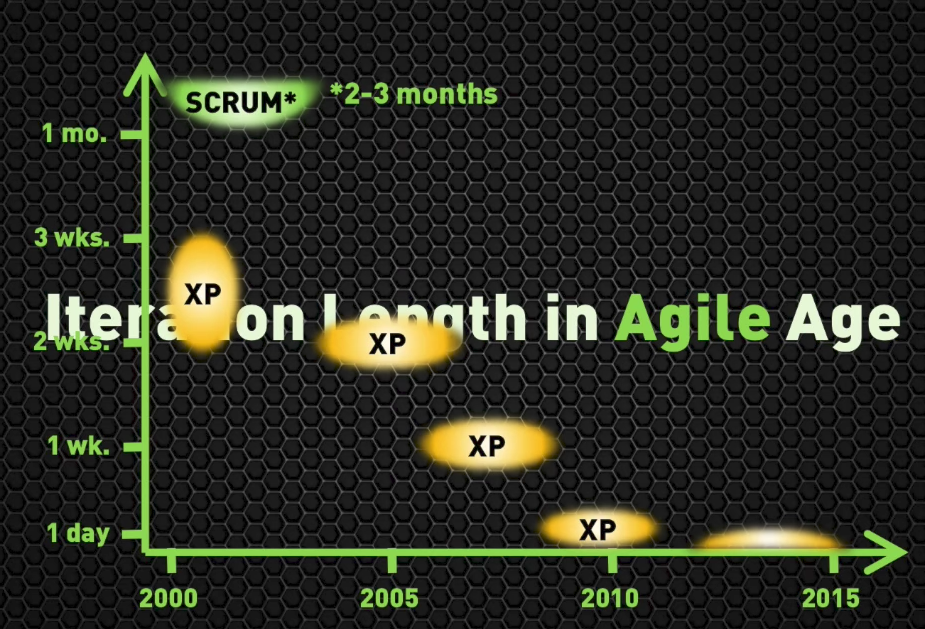
\includegraphics[scale=0.2]{introduction_iteration_agile_age}  
  \caption{Iteration length in the agile age}
  \label{fig:introduction_iteration_agile_age}
\end{figure}



\note{
There is material in his speech to go on here. Talk more about the pyramid of 'interaction level' with customers that he shows.
}

Eric Evans talked about domain driven design (DDD) at the \textit{Domain Driven Design Europe} conference\cite{evans2016tackling} in 2016, focusing on the role of DDD in state of the art development. Evans explains how available development technologies have diversified, and developer insight and knowledge is very good. Monolith applications were a result of technological boundaries, and prohibited good design of big applications. According to Evans these boundaries have disappeared, pushing developers towards more thoughtful design of applications. By creating monolith applications, development of a clearly separated applications is really hard. Developers today need to put emphasis on understanding the underlying challenges in the particular domain, identifying the optimal architecture that supports the context.



\comment{Kunne man snakke om at der er kommet en meget større mediator? Mange flere resourcer for moderne developers.}

\note{
We need need another architecture

How do we break down the problems
How do we create and architecture that gives us the possibility to work fast, in independently teams
Where did we come from, where do we want to go

\begin{figure}[!htb]
  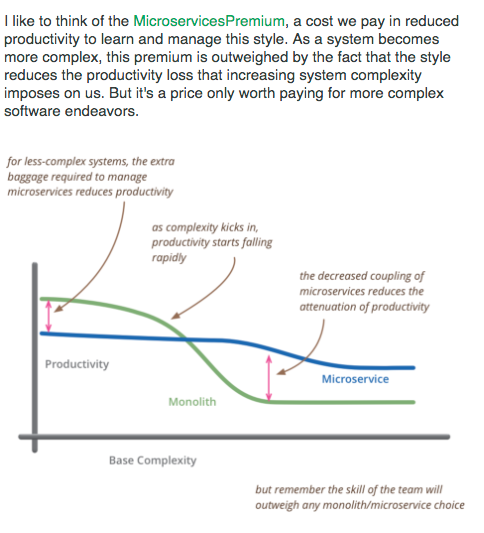
\includegraphics[scale=1]{introduction_microservice_premium}  
  \caption{The microservice premium}
  \label{fig:introduction_microservice_premium}
\end{figure}

}

\note{
Technology makes us able to achieve more things

Cloud computing has introduced virtualization, makes it possible to do new cool things

Knowledge sharing has increased exponentially. Open source frameworks, and tools.
A defining characteristic of NoSQL is open source. - Is taken from the fowler book
Kubernetes, Kafka, Cassandra
}

\note{
Challenges in this new space

}
\note {
\section{It not just microservices}
Several movements have started based on working processes, software architectures and technology. There are entire conferences based on these particular topics, there among microservices, agile, NoSQL, Cassandra and more. These George calls these \textit{industry "Hot" topics}. These topics are all based around going faster, as a company, when creating, updating and expanding applications. 

The problem domain has changed, problems today are very complex. When starting to solve a problem, you start in a state of disorder, where the problem has to be defined. Todays application work on these problems, because that is where the value is according to George.

Competition is very fast, new technology enables start up companies to move fast. Cloud computing gives the possibility to reserve resource, immediately, easy and cheaper than ever before. These cloud solutions also drive down barriers for entering global markets, a infrastructure is easily created on the other side of the world. Many programming languages are available, and supported by frameworks that makes it possible to create something functional very quickly. These things are open source and easily available to start up companies.

\textbf{Scrum and Delivery cycles}
Scrum iteration time has been cut drastically in time. A iteration time of 2 or 3 weeks is too long according to George. Delivery cycles has been reduced from 5 or 3 years in the 1980's, to 1 week or a single day in 2015. This has been achieved by optimizing the work process.

There are three type of inhibitors, technology, process and organisational explained below.

\subsection{technology inhibitors}
\textbf{Cloud exploitation}
Cloud computing and containerization has made it possible to order hardware very quickly. Docker has made it possible to start a new container in 5 seconds. Capacity planning, estimating the needed capacity before beginning developing an application is now useless. With virtualization it has become a operational expense. This is hard to change in big companies, has a lot to do with the organisation.

Services can now be developed very small, instead of having a single big service, containing more than a million lines of code, services can now consist of only 50 lines of code. This is possible because of virtualization. Several very successful big scale companies, has moved in this direction independently.

\textbf{Programming languages}
Event busses is a key factor in making microservices a thing. Traditionally you would have a SQL database, with operational data in it, there would be scripts build around updating and testing it.
Event buses substitute this by introducing a stream that can publish events pushed to it. By implementing services that subscribe to this event bus and filters the messages, a publish/subscribe pattern can be achieved. Services can subscribe to events in the cluster that are interesting to them, and react accordingly. Services publish their events on to the event bus, when they have results that are interesting for other parts of the cluster.
LinkedIn uses Kafka, and has opensourced it.

By building systems as microservices, the system architecture changes drastically. When systems need help from other services, it is published to the event bus, subscribing 'helper' services then react on the incoming event, if they are needed. This isolates the services, they are only responding to events, further several service version can be run in parallel, updating a service without stopping the old version before dependent services have migrated to the new one. If one type of service fails, the dependent service can degrade functionality gracefully.

Incremental applications are made available through this event bus. Services can be added as they are developed. As services are added, functionality rises. Developed code earns money immediately. Improving development speed.

Big database is dead. The eventbus holds anything interesting. If you need persistence, hold your own copy of the information. We prefer to cache the data locally than query the remotely. Database poly-glot, each service can hold the data it needs. This makes us faster, we can choose the database we need.

You want to put everything on the eventbus. Not only communication between services but also user stories, logging, server status and so on. You therefore need the rivers of the main river.

\textbf{Open source frameworks}
Netflix has open sourced a lot of their libraries. Docker is open source. Do not be afraid of using it.

Disruptive languages are coming in. A lot of different languages are being used now. Some of them are really good at a specific job we solved in forexmaple java before. Now can be solved in 4000 instead of 130.000 lines of code. Scala, Erlang, Clojure are functional languages being used now.


\subsection{Process inhibitors}
\textbf{Problem}
You have to figure out which problem you are trying to solve. If you are solving a complex problem microservices are good. If you are solving a straightforward problem, traditional architecture may be better.

\textbf{Requirements}
It is hard to solve complex problems. We cannot set requirements for that, no one know how to achieve it. We want to know what we want to accomplish with the application. How do you make money, how do you get ore clicks. We want to experiment different implementations. Experimentation drives innovation, we want to fail and learn from it. 

\textbf{Interaction with customers}
Customers come and tell us what features need to be. Teach the developer their domain. Raise up to the feature level, figure out how to solve the problems presented by the customers.

\textbf{Measure what matters}
Business success metrics. Measure programmers against that. 

\subsection{Organisational inhibitors}
\textbf{Over specialization}
Too many titles. 

Project managers, team leads were removed. 

Made simple model, you can be a graduate, developer or senior developer and System developer(Full stack developer) at the same level. System developers was the wanted goal. They can be handed feature requests and figure out how it should be implemented.

\textbf{Fix the furniture}
You sit at the same table as the rest of the feature team.

\textbf{Dedicated leadership was killed}
Leadership was removed from each team. There is no need for a dedicated leader to lead 10 people team.
Leaders would do the same as the other workers, if the leader was needed, you go talk to him.

\textbf{Bringing work to the team}
There is a tendandncy to reform projects and put programmers together and that defines the new team.
It takes 4-7 weeks before the team is productive, agree on technology and communication tools. Teams are therefore not reformed.
Come with project and money to our team, and we will implement it, until you do not have more money.

\subsection{Take away}
You need to do all of these things to be successful with microservices. You can deliver very fast if you are able to make it.
}

\note{

\section{Time is ripe}
Eric Evans talked about domain driven design (DDD) at the 'Domain Driven Design Europe' conference\cite{evans2016tackling}, focusing on the role of DDD in state of the art development. Evans explains how available development technologies have diversified, and developer insight and knowledge in available technologies is high. Evans describes the status of the software development community in 2003 when he wrote his well known book: \textit{Domain Driven Design Tackling Complexity in the Heart of Software}\cite{evans2004domain}. According to Evans software developers were not necessarily ready to put focus on DDD in 2003. The amount of broadly used languages, was limited to Java and J2EE, with SQL as the only available database technology. Applications at that time always utilizing these languages. Evans emphasise how software developers were focused on learning to utilize programming languages, where as today's developers have a deep understanding languages and tools, and are ready to utilize them. Developers today can afford to put emphasis on understanding the underlying challenges in the particular domain, and finding the optimal architecture to solve them. DDD is too hard to accomplish with previous limitations, but a new level of seasoned development languages, frameworks and tools together with a higher skill level amongst programmers now makes DDD viable for everyone. According to Evans It is a good time to take DDD to the next level, different technology movements are pushing developers towards more thoughtful design of applications. Developers cannot get away with the same amount of sloppiness, because modern applications cannot be compiled into a single server side monolith. Evans further states that there are big rewards for small loosely coupled modules, having clear cut and limited functionality, and that these rewards are necessary for successful development of modern applications.

}

\note {
Object oriented programming was the only modelling paradigm beforehand. Event sourcing is another and newer paradigm. Relational is a modelling paradigm, that makes it possible compare and manipulate big sets of data. Relational schemas has been used as generalised places to put all data in an application. 
We want to create a schema that takes just the data we need.

"A feature common to the successes was a rich domain model that evolved through iterations of design and became part of the fabric of the project." \cite[Preface]{evans2004domain}
“model represents some aspect of reality or an idea that is of interest. A model is a simplification. It is an interpretation of reality that abstracts the aspects relevant to solving the problem at hand and ignores extraneous detail." \cite[p.~2]{evans2004domain}

“It excluded hundreds of facts that the engineers understood but that were not directly relevant, such as the actual digital features of the components.” \cite[p.~12]{evans2004domain}

“He or she would have a framework to organize new information and learn faster, to make better guesses about what was important and what was not, and to communicate better with the PCB engineers.”\cite[p.~12]{evans2004domain}

“Effective domain modelers are knowledge crunchers. They take a torrent of information and probe for the relevant trickle.”\cite[p.~13]{evans2004domain}

“This distillation is a rigorous expression of the particular knowledge that has been found most relevant.”\cite[p.~13]{evans2004domain}
}

\note {

\section{Microservices at Netflix scale}
Netflix are very known for utilizing microservices at a monumental scale, and are often quoted and set as an example for the movement towards microservice architectures. In a talk at \textit{GOTO Amsterdam 2016}, called \textit{Microservices at Netflix Scale: Principles, Tradeoffs \& Lessons Learned}\cite{meshenberg2016microservices} with Ruslan Meschenberg, director of Platform engineering at Netflix. 




There are challenges with doing microservices.

Their old monolith application could not be moved directly to the cloud. Therefore they piece by piece moved it to the cloud.

Monolith was latent to bugs, introducing a bug in one part, the bug was in the entire application. The RDBMS was further a single point of failure. Not very resilient.
They had a meltdown of their delivery system, which caused them to prioritize moving from a monolith to microservices.

\subsection{First principles of microservices}
\textbf{Buy it vs build it}
Netflix does only build software if they have to, and cannot use open source or payed software. Put emphasise on contributing to open source is in focus contra buying software.

\textbf{Services should be stateless}
Most of your services should be stateless, exception for persistence and caching layer.
If a node die, you just need to retry it or hit another instance.
Netflix use caos testing to prove they do this.

\textbf{Scale out vs. up}
If you keep scaling up, you hit a limit.
Horizontal scaling gives a longer runway. It is so much easier to add new instances. Cloud gives the benefit of elasticity.

\textbf{Redundancy and isolation for resiliency}
You do not want a single point of failure.
We want to isolate failures, so we do not get cascading failures. Then redundancy does not necessarily help.

\textbf{Automate destructive testing}
Simian Army. Started with chaos monkey.
Our system will fail, and it will fail at a suboptimal time, if we do not develop a resilient system.

\subsection{Principles in action}
\textbf{Stateless services}
In order for a stateless service to be a good citizen. Register in service discovery. Needs to implement a health check, so external system can verify it is functional. If it wants to call other services it needs to call service discovery to get information on the other service locations.

You need to test that services are stateless while they are running in production. Development environment will not be the same.

\textbf{Chaos monkey}
Runs around and destroys services, monday to friday.

\textbf{Data}
From RDBMS to Cassandra.

Cassandra is Netflix main key value storage.
It is one of the biggest scale noSQL services. It is open source, Netflix needed to contribute, making it multi regional, multi directional replication ready.
Storage engine, with respect to CAP theorem, available, partition tolerance, tunable consistency. 

\textbf{Billing services}
Deal with money, and they have to be a bit more careful. Want to do it just right. 
It needs to be fully locked, and is not as accessible as the rest of the services.
Took Netflix the longest to migrate to the cloud, of all their services from the monolith.


\subsection{Priorities}
\textbf{1. Innovation}
Always strive for innovation, traded for reliability and efficiency.

\textbf{2.Reliability}


\textbf{3. Efficiency}

Challenge in monolith, there is a lot of coupling between teams, one team may be ready for deploying, others are not. It is too slow, hinders the innovation.

Loose coupling: Each team work independently. Each team Develop, Test, Deploy and support their product. End-end ownership.
There is a motivation for writing quality code, and writing it fast. Engineers get motivated by results and their impact. Everyone are constantly doing something.

Separation of concerns:
Each team can focus on their core.

\subsection{Cost of microservices}
\textbf{Changes the organisation}
Some jobs disappear.

You want to evolve the organisation.

\textbf{Migration does not happen overnight}
It takes time before you can move everything to the new system. Have to maintain and possible expand the old monolith.

\subsection{Lessons learned}
\textbf{IPC is crucial for loose coupling}
Common language between the services, establish the contract/language between services.

You want some homogeneity how you deploy the services. People do not have to reinvent how the deploy the applications.
Gives source of truth, if something goes wrong, we can look at which technology we changed lastly.

\textbf{Databases}
Caching to protect DBs

500 plus microservices are harder on the database than one or two monoliths.
Therefore netflix uses chaches in front of the databases.

\textbf{Telemetry}
Operational visibility matters.

Will telemetry scale with number of services, and will you be able to identify what is important to monitor.
Observe -> Orient -> Decide -> Act
This is done automatically, there is to many logs for a human to make any sense of.

\textbf{Arkitektural diagram}
You do not have the luxury of a architecture diagram. You have to create diagram at runtime, because changes in the architecture happens all the time.

\textbf{Reliability matters}
It is really important at scale.
Rate of failure is proportional to the amount of change at the scale at which the system is running. Netflix are pushing a lot of changes and are running at massive scale.

Netflix strive for 4 9's of availability. 52 minutes of downtime a year.

\textbf{Availability}
Availability is very important. Netflix likes to focus on Innovation and velocity, but availability is important to retain customers.

Cascading failures are prone in microservices. If each microservices has a availability of 99.99, the overall availability gets poor.
We want to detect and correct the errors. Therefore we use circuit breakers, because we do not want to propagate the failure to the client. 
We want to figure out if the failure is in a non-critical service. If it is not critical we can probably still give good service in the remaining areas.

\textbf{Destructive testing}
You have to inject failure in production. Not to start with, but in the end.

FIT - Fault-injection Test Framework, used to insert failures into http connections, 'test harness'.

\textbf{Containers}
Does not make microservices.

Changes the level of encapsulation, from virtual machine to process.
Great benefits for developer velocity, iterate on short cycles, you can do a lot of cool things. It is not a silver bullet.
Running containers at scale requires a very good infrastructure. Use kubernetes if you want to run it.

\subsection{Microservices resource}
\textbf{Netlfix made a lot of open source}
Use it instead of developing it on your own.

\subsection{Take away}
Microservices bring good value. To developer velocity, availability and other dimensions.

They are not free. It requires orginisational changes and central infrastructure investment. Do not necessarily do it just because Netflix did it.

}

\note{

\section{Abstraction}
Here we want to discuss how we see a modern cloud native application.
We want some kind of diagram that shows our perspective. Which layers and how will we distinguish here on out.

We want the cloud native diagram one, with all technologies in it.

“Most SERVICES discussed in the literature are purely technical and belong in the infrastructure layer. Domain and application SERVICES collaborate with these infrastructure SERVICES. For example, a bank might have an application that sends an e-mail to a customer when an account balance falls below a specific threshold. The interface that encapsulates the e-mail system, and perhaps alternate means of notification, is a SERVICE in the infrastructure layer."\cite[p.~103]{evans2004domain}
}

\newpage

\section{Problem formulation}
\label{sc:problem_formulation}

\begin{itemize}  
\item 1.a How can cloud computing be used to solve availability, performance and maintainability requirements for enterprise applications?
\item 1.b How can cloud computing be used in an enterprise application architecture?

\item 2.a How are enterprise application challenges and possible solutions affected by the application domain?
\item 2.b How does the enterprise application domain affect challenges and possible solutions?
\item 2.c How does the domain shape the challenges in a specific application architecture?
\item 2.d How does the domain and organization shape the challenges in a specific application architecture?

\item 3.a How does a distributed application architecture deal with a single point of failure?
\item 3.b How is single point of failure avoided in a distributed application architecture?

\item 3.c How is the optimal application architecture and distribution method determined and evaluated?
\item 3.d How is the enterprise application architecture determined?
\item 3.e How is the enterprise application architecture evaluated?
\end{itemize}

\subsection*{Notes}
How are the challenges and their optimal solution affected by the specific application?

What determines the optimal application architecture, database and distribution?

How is the optimal application architecture, database and distribution determined?

System architecture:
How is application data optimally stored?
How is application data optimally distributed?

How are application updates optimally executed?
How are updates 

How is the system distributed

This area has been named cloud computing, 

Big cloud computing platforms are now available, offering server rental with 

From these requirements big cloud platforms have been started, 

These requirements has started big scale initiatives in cloud computing, has generated new tools and databases available for development of distributed big scale enterprise applications. 

Creating a need for developers to explore and evaluate which of the many platforms to choose, 

\note{

Kig i kapitel 2 s. 59 - cloud-native-java-designing-resilient-systems-with-spring-boot-spring-cloud-and-cloud-foundry
"The patterns for how we develop software, both in teams and as individuals, are always evolving. The open source software movement has provided the software industry with somewhat of a Cambrian explosion of tools, frameworks, platforms, and operating systems—all with an increasing focus on flexibility and automation. A majority of today’s most popular open source tools focus on features that give software teams the ability to continuously deliver software faster than ever before possible, at every level, from development to operations."

\subsection*{Noter}
These requirements has started big scale initiatives in cloud computing, has generated new tools and databases available for development of distributed big scale enterprise applications. 

Creating a need for developers to explore and evaluate which of the many platforms to choose, 

has generated new tools and databases available for development of distributed big scale enterprise applications.

platform for automating deployment, scaling, and operations of application containers across clusters of hosts

Which level are we on? High level: Google app engine, or low level abstraction: EC2.

"The Antifragile Organization" - \url{http://queue.acm.org/detail.cfm?id=2499552}
"Failure is inevitable. Disks fail. Software bugs lie dormant waiting for just the right conditions to bite. People make mistakes. Data centers are built on farms of unreliable commodity hardware. If you're running in a cloud environment, then many of these factors are outside of your control. To compound the problem, failure is not predictable and doesn't occur with uniform probability and frequency. The lack of a uniform frequency increases uncertainty and risk in the system. In the face of such inevitable and unpredictable failure, how can you build a reliable service that provides the high level of availability your users can depend on?"

Why is it worth it to take on this monster of instability?


"Weathering the Unexpected" - \url{http://queue.acm.org/detail.cfm?id=2371516}

"Whether it is a hurricane blowing down power lines, a volcanic-ash cloud grounding all flights for a continent, or a humble rodent gnawing through underground fibers—the unexpected happens. We cannot do much to prevent it, but there is a lot we can do to be prepared for it. To this end, Google runs an annual, company-wide, multi-day Disaster Recovery Testing event—DiRT—the objective of which is to ensure that Google's services and internal business operations continue to run following a disaster."


Disasters happen for all kinds of systems. So lets prepare for it already in implementation.


"Site Reliability Engineering" - (page 17 in downloaded pdf)

"Software engineering has this in common with having children: the labor before the birth is painful and difficult, but the labor a er the birth is where you actually spend most of your effort. Yet software engineering as a discipline spends much more time talking about the first period as opposed to the second, despite estimates that 40–90% of the total costs of a system are incurred after birth.1"


Software systems incur a lot of work even after deployment, so lets spend some time here.



"Toward Antifragile Cloud Computing Infrastructures"\cite{abid2014toward}
"Cloud computing systems are rapidly growing in scale and complexity. They are also changing dynamically as a result of dynamic addition and removal of system components, different execution environments, common updates and upgrades, runtime repairs, mobility of devices and more. Such large-scale, complex and dynamic cloud environments are prone to failures and performance anomalies"


"Resilience and Survivability in Communication Networks: Strategies, Principles, and Survey of Disciplines"\cite{sterbenz2010resilience}
"The Internet has become essential to all aspects of modern life, and thus the consequences of network disruption have become increasingly severe. It is widely recognised that the Internet is not su ciently resilient, survivable, and dependable, and that significant research, development, and engineering is necessary to improve the situation."

"Networks in general, and the Global Internet in particular, have become essential for the routine operation of businesses and to the global economy. Consumers use the Internet to access information, obtain products and services, manage finances, and communicate with one another. Businesses use the Internet to transact commerce with consumers and other businesses."



"Toward Antifragile Cloud Computing Infrastructures" "Amal Abida,b, Mouna Torjmen Khemakhema, Soumaya Marzouka, Maher Ben Jemaaa, Thierry Monteilb,c, Khalil Drirab,c"
"Cloud computing is earning an increasing popularity over traditional information processing systems for storing and processing huge volumes of data. This concept consists in offering services and resources on-demand over the Internet in the pay-as-you-go model. The Cloud infrastructure is built on modern data centers covering thousands of interconnected servers with capability of hosting a large number of applications. These data centers are often virtual- ized and computing resources are provisioned to the user in the form of configurable Virtual Machines (VMs)."



Stability summary chapter 6 \cite[p. 117]{nygard2007release}

"Astronomically unlikely coincidences happen daily"
"Failures are inevitable. Our systems, and those we depend on will fail in ways large and small. Stability antipatterns amplify transient events. They accelerate cracks in the system. Avoiding the antipatterns does not prevent bad things from happening, but they wull help minimize the damage when bad things do occur."


"A View of Cloud Computing"
"While the cost of over provisioning is easily measured, the cost of under provisioning is more difficult to measure yet potentially equally serious: not only do rejected users generate zero revenue, they may never come back"
"In fact, this example underestimates the benefits of elasticity, because in addition to simple diurnal patterns, most services also experience seasonal or other periodic demand variation (for example, e-commerce in December and photo sharing sites after holidays) as well as some unexpected demand bursts due to external events "
}

\note{
“1.4. Attack of the Clusters
At the beginning of the new millennium the technology world was hit by the busting of the 1990s dot-com bubble. While this saw many people questioning the economic future of the Internet, the 2000s did see several large web properties dramatically increase in scale.”
Excerpt From: “NoSQL Distilled: A Brief Guide to the Emerging World of Polyglot Persistence.” 


“One is to handle data access with sizes and performance that demand a cluster; the other is to improve the productivity of application development by using a more convenient data interaction style”
Excerpt From: pramod j. sadalage. “NoSQL Distilled: A Brief Guide to the Emerging World of Polyglot Persistence.” iBooks.
}






